% ============================================================
% File:    job_talk_robustness.tex
% Purpose: job_talk.tex plus the 2026-09-23 k=2 results: two-instrument
%          (upstream + downstream mines) 2SLS, event-study pre-trends, and
%          regressor-swap robustness (annual production / mine count),
%          which replace the watershed-radius (k-grid) robustness slides
% Inputs:  ../../output/reg/*_present.tex, ../../output/sum/*_present.tex,
%          ../../output/fig/*.png, img/*, citation.bib
% Outputs: job_talk_robustness.pdf
% Author:  EK  Date: 2026-09-23
% ============================================================

\documentclass{beamer}
\usetheme{Boadilla}
\setbeamertemplate{footline}[page number]
\setbeamertemplate{navigation symbols}{}

\usepackage{graphicx}
\usepackage{booktabs}
\usepackage{array}
\usepackage{adjustbox}
\usepackage{varwidth}
\usepackage{amsmath}
\usepackage{amssymb}

\usepackage[
backend=biber,
style=authoryear,
citestyle=bwl-FU
]{biblatex}
\addbibresource{citation.bib}

% ============================================================
% Pipeline output directory (relative to this file)
%   \presreg{name}  -> ../../output/reg/name_present.tex
%   \pressum{name}  -> ../../output/sum/name_present.tex
%   \presfig{f.png} -> ../../output/fig/f.png
% ============================================================
\newcommand{\outputdir}{../../output}

% The generated *_present.tex files are written as article floats:
% \begin{table}[htbp] ... \caption{...} ... \end{table}. Beamer has no float
% mechanism, and wrapping a float in adjustbox raises
% "! LaTeX Error: Not in outer par mode." Neutralise the float and swallow the
% caption (on a slide the frame title carries the caption text), so the table
% body is plain material that can be boxed and scaled.
\makeatletter
\renewenvironment{table}[1][]{\par\centering}{\par}
\renewcommand{\caption}[2][]{}
\makeatother

% Box the table body at its natural width inside a varwidth, so multi-panel
% files still break between panels instead of setting them side by side, then
% shrink only as much as is needed to fit the slide.
% Optional argument overrides the width key, for source files that hardcode a
% narrow adjustbox (e.g. width = 0.45\textwidth) and so need scaling UP: max
% width only ever shrinks.
\newcommand{\slidetableinput}[2][max width=\textwidth]{%
  \adjustbox{#1, max totalheight=0.80\textheight, center}{%
    \begin{varwidth}{17cm}%
      \input{#2}%
    \end{varwidth}}}
\newcommand{\presreg}[2][max width=\textwidth]{\slidetableinput[#1]{\outputdir/reg/#2_present}}
\newcommand{\pressum}[2][max width=\textwidth]{\slidetableinput[#1]{\outputdir/sum/#2_present}}
\newcommand{\presfig}[2][0.75\textheight]{%
  \begin{center}%
  \adjustbox{max width=\textwidth, max height=#1}{\includegraphics{\outputdir/fig/#2}}%
  \end{center}}

% One-line takeaway under a table or figure. The group must close AFTER \par or
% the paragraph inherits the outer font's baselineskip on its first line.
\newcommand{\takeaway}[1]{\par\medskip{\footnotesize #1\par}}

% In-text link to a backup/appendix slide. #1 = \hypertarget name on the
% backup frame, #2 = short description of what the link shows.
\newcommand{\backuplink}[2]{\hyperlink{#1}{\footnotesize(#2 $\rightarrow$)}}

% Underbrace whose label wraps to the width of the braced math, so long labels
% sit under their own term instead of running across the slide.
% #1 = braced math (typeset in display style), #2 = label text.
\newlength{\ubwidth}
\newcommand{\ubtext}[2]{%
  \settowidth{\ubwidth}{$\displaystyle #1$}%
  \underbrace{#1}_{\parbox[t]{\ubwidth}{\centering\scriptsize #2}}}

\AtBeginSection[]{
  \begin{frame}
  \vfill
  \centering
  \begin{beamercolorbox}[sep=8pt,center,shadow=true,rounded=true]{title}
    \usebeamerfont{title}\insertsectionhead\par%
  \end{beamercolorbox}
  \vfill
  \end{frame}
}

\title[Contamination and Self-Reported Compliance]{The Effect of Contamination on Contamination Limit Regulation}
\subtitle{US Coal Mining and Drinking Water Utilities}
\author{Emil Kee-Tui}
\institute{Charles H. Dyson School of Applied Economics and Management \\ Cornell University}
\date{September 2026}

\begin{document}

% ---------------------------------------------------------------- 1
\begin{frame}
\titlepage
\end{frame}

\begin{frame}{Self-reported compliance}
\begin{itemize}
    \item Regulatory models requiring entities to self-report compliance:
    \begin{itemize}
        \item Healthcare HIPAA violation disclosure; Energy firms self-report anti-competitiveness/negligence to the Federal Energy Regulatory Commission; Public companies' SOX self-report financial statement accuracy; Drinking water utilities' water quality.
    \end{itemize}
    \item Incentive to shirk reporting. Consider drinking water utilities' federal water quality regulation:
    \begin{itemize}
        \item No self-report $\Rightarrow$ no contamination exceedance violation issued \parencite{naylor5537637strategic, zou2021unwatched}.
        \item No self-report saves self-reporting costs \parencite{oleckno1982national}.
    \end{itemize}
    \item \textbf{Incentives rise with contamination}
    \begin{itemize}
        \item $\uparrow$ contamination $\rightarrow \uparrow$ testing requirements ($\uparrow$ \textbf{reporting costs})
        \item $\uparrow$ contamination $\rightarrow \uparrow$ probability contamination violation ($\uparrow$ \textbf{need to conceal}).
    \end{itemize}
    \item Whether it is self-reporting costs or concealment has different policy implications for improving reporting.
\end{itemize}
\end{frame}

\begin{frame}{Drinking water quality and coal mining}
\begin{itemize}
    \item Drinking water utilities provide treated water to 85\% of US households.
    \begin{itemize}
        \item Utilities source from groundwater and/or surface water, serve from twenty-five to millions of customers, publicly or privately owned.
    \end{itemize}
    \item 9 to 34 million US households obtain water from a utility violating a health standard \parencite{allaire2018national}.
    \item \textbf{Coal mining is a source of water contamination} 
    \begin{itemize}
        \item \textbf{Acid mine drainage}: sulfuric acid formed from sulfide rock dissolves metal ions and sulfates, travels into surface and ground water \parencite{skousen2019acid}.
        \item \textbf{Coal wash slurry}: impurities stored in retaining ponds seep through porous rock, or ponds fail.
    \end{itemize}
    \item Federal policy is expanding mining access and delaying plant retirements (\cite{Trump2025EO14260}; \cite{Daly2025CoalMining}).
    \item Coal supplied 16\% of US electricity in 2025 (\cite{IEA2025GER}).
    \end{itemize}
\end{frame}

% ---------------------------------------------------------------- 4
\begin{frame}{Research questions}
\begin{center}
\begin{beamercolorbox}[sep=10pt,center,rounded=true,shadow=true]{block body}
\large Does coal mining raise contamination at drinking water utilities?
\end{beamercolorbox}
\end{center}

\begin{center}
\begin{beamercolorbox}[sep=10pt,center,rounded=true,shadow=true]{block body}
\large What happens to firm self-reporting when contamination rises exogenously, under self-reported compliance?
\end{beamercolorbox}
\end{center}

\begin{center}
\begin{beamercolorbox}[sep=10pt,center,rounded=true,shadow=true]{block body}
\large Is any reduction in self-reporting concealment of exceedances, or avoidance of reporting costs?
\end{beamercolorbox}
\end{center}
\end{frame}

% ---------------------------------------------------------------- 5
\begin{frame}{What I do}
\begin{itemize}
    \item Setting: drinking water utilities downstream of coal mines, 1985--2005.
    \begin{itemize}
        \item Contamination is an \textbf{upstream externality} --- the firm cannot reduce it by cutting output \parencite{bennear2005strategic}.
        \item Separating contamination from utility choices helps identify the effect of contamination.
    \end{itemize}
    \item Adapt \textcite{stratford2015coalprod} instrument for coal production to address two sources of endogeneity:
    \begin{itemize}
        \item Coal mines are near coal seams and transportation that independently predict water quality and utility characteristics.
        \item Regulators block upstream mining for vulnerable utilities.
    \end{itemize}
    \item Contributions:
    \begin{itemize}
        \item Causal evidence that contamination reduces self-reporting.
        \item Rationalize utility decisions to self-report in light of regulator's actions with a model.
        \item First evidence that \textbf{the cost of self-reporting}, not only concealment, causes environmental under-reporting \parencite{naylor5537637strategic, zou2021unwatched}.
        \item First causal estimates of the effect of \textbf{coal mining on treated drinking water} at US utilities.
    \end{itemize}
\end{itemize}
\end{frame}

% ---------------------------------------------------------------- 6
\begin{frame}{What I find}
\begin{itemize}\small
    \item $\uparrow$ mining $\rightarrow$ $\uparrow$ contaminant concentrations, but never above the MCL. 10M cumulative tons upstream raises mean nitrate by 11.0\% of its sample mean (***) and selenium by 8.5\% (**); arsenic and barium show no significant change.
    \item $\uparrow$ mining $\rightarrow$ $\uparrow$ \textbf{under-reporting}. One more upstream mine raises MR violations by 3--5 pp, against base rates of roughly 4--6\%.
    \item $\uparrow$ mining $\rightarrow$ \textbf{no significant change} in MCL violations.
    \item $\uparrow$ mining $\rightarrow$ $\uparrow$ \textbf{inspection visits} ($+$2.1 pp).
    \item Formal enforcement: $-$3.4 pp with utility and year fixed effects, $-$1.1 pp (not significant) with state $\times$ year fixed effects, against a base rate of 3\%.
    \item \textbf{Self-reporting costs, not concealment}: 
    \begin{itemize}
        \item When nitrate readings cross 50\% of the MCL $\rightarrow$ monitoring requirements $\uparrow$ (reporting cost $\uparrow$) $\rightarrow$ self-reporting $\downarrow$.
        \item Sanitary inspections at under-reporting utilities do not discover concealed violations.
        \item Contaminant concentrations stay below MCL.
    \end{itemize}
\end{itemize}
\medskip
\begin{center}
\begin{beamercolorbox}[sep=6pt,center,rounded=true]{block body}
Contamination shifts monitoring from the firm onto the regulator.
\end{beamercolorbox}
\end{center}
\end{frame}

% ================================================================
\section{Self-reporting model}
% ================================================================

% ---------------------------------------------------------------- 8


% ---------------------------------------------------------------- 10

\begin{frame}{Institutional setting}
\begin{itemize}
\item Utilities federally regulated by the Safe Drinking Water Act (``SDWA'').
\item Contaminants cannot exceed a Maximum Contaminant Level (``MCL'').
\item Self-report to regulator or get a Monitoring and Reporting violation (``MR'').
\item Self-reporting requirements depend on water contamination/threats to water.
\item States are SDWA enforcers with discretion over enforcement and visits:
\begin{itemize}
    \item Sanitary survey - comprehensive on-site inspection
    \item Technical assistance - helps fix problem or become compliant.
    \item Sampling - prompted by suspected contamination event or violation.
    \item Enforcement visit - triggered by suspected violation.
\end{itemize}

\item Enforcement, while remedial rather than punitive, is still costly:
\begin{itemize}
    \item Informal (letters, notices, compliance plans)
    \item Formal (consent decrees, fines, prosecution)
    \item MR violations are punished less severely than MCL violations.
\end{itemize}
\end{itemize}
\end{frame}




% ---------------------------------------------------------------- 11
\begin{frame}{Model: the utility's decisions to self-report or under-report}
Utility draws compliance cost type $\theta \sim F(\cdot\,;m)$, worsening in upstream contamination $m$.
\begin{itemize}\small
    \item Choose negligence $a$, unobserved by regulator, with benefit $\theta b(a)$
    \item Opportunity cost relative to a maximum negligence $\theta b(\bar{a})$.
    \end{itemize}
 Utility draws a self-reporting cost $c \sim G(\cdot\,;m)$, worsening in upstream contamination $m$.
 \begin{itemize}
    \item A test reveals an MCL with probability $q(a)$, $q'\geq0$.
\end{itemize}
\end{frame}

\begin{frame}{Model: the utility's decisions to self-report or under-report}

Penalties: $r$ for a self-reported exceedance, $t$ for an MR violation, $s>r$ if an inspection (probability $p$) uncovers a hidden exceedance.

\[
\underbrace{c + q(a)\,r}_{\text{report}} \;\lessgtr\; \underbrace{t + p\,q(a)\,s}_{\text{under-report}}
\;\Longrightarrow\;
\text{report iff } c \le \hat c(a) \equiv t - (r-ps)\,q(a).
\]
\begin{itemize}
    \item A system with \textbf{zero} exceedance risk still stops reporting once $c > t$.
\end{itemize}

\[e(a;c) = \min\left\{\, c + q(a)r,\;\; t + \,q(a)ps \,\right\}\]
\begin{itemize}
    \item The utility chooses $a$ to maximize $-\theta[b(\bar{a})-b(a)] - e(a; c)$.
\end{itemize}
\end{frame}

% ---------------------------------------------------------------- 12
\begin{frame}{Model: why the utility under-reports}
\begin{block}{Proposition 2}
A type-$\theta$ utility under-reports if and only if its cost draw exceeds this cutoff, $c > c^*(\theta)$, so the share of utilities under-reporting and receiving an MR violation is:
\[
MR(m) = \int_0^{\bar\theta} \big[\,1 - G(c^*(\theta);m)\,\big]\, f(\theta;m)\, d\theta \;\equiv\; \int_0^{\bar\theta} h(\theta,m)\, f(\theta;m)\, d\theta.
\]
Differentiating splits into two channels:
\[
\frac{\partial MR}{\partial m} = \ubtext{\int_0^{\bar\theta} \frac{\partial h(\theta,m)}{\partial m}\, f(\theta;m)\, d\theta}{Channel A: cost-distribution shift. Hold $\theta$ distribution fixed and change probability type $\theta$ utilities draw $c$ exceeding $c^*$} \;+\; \ubtext{\int_0^{\bar\theta} h(\theta,m)\, \frac{\partial f(\theta;m)}{\partial m}\, d\theta}{Channel B: type-distribution shift. Hold proportion of type $\theta$ utilities whose cutoff exceeds $c^*$ fixed and change the proportion of utilities of type $\theta$.}
\]
\end{block}
\end{frame}

% ---------------------------------------------------------------- 13
\begin{frame}{Data}
\begin{itemize}\small
    \item \textbf{Violations, enforcement, visits} --- SDWIS/ECHO, universe of utilities 1985--2005. Binary by utility $\times$ year; days-in-year as a robustness measure.
    \begin{itemize}
        \item Under-inclusive but accurate: 95\% of the violations SDWIS holds are correctly reported (US EPA, 2000).
    \end{itemize}
    \item \textbf{Contaminant concentrations} --- EPA Six-Year Review round 2, 1998--2005. Cleaned following \cite{ravalli2022sociodemographic}; non-detects set to MDL/$\sqrt{2}$.
    \item Contaminants: \textbf{arsenic, nitrate, barium, selenium} --- inorganic chemicals with stable utility MCLs 1985--2005.
    \item \textbf{Mines} --- MSHA locations merged to EIA annual production, mine level.
    \item \textbf{Coal sulfur \%} --- USGS COALQUAL samples, averaged within 20 km of each watershed.
    \item \textbf{Hydrology} --- NHDPlus HUC12 watershed boundaries and inflow/outflow.
    \item \textbf{Sample}: Utilities with a coal mine \textbf{within two watersheds upstream} of their intake and no coal mine colocated with their intake. 10,641 utility-years, 565 utilities.
\end{itemize}
\end{frame}

% ---------------------------------------------------------------- 14
\begin{frame}{Matching intakes to the watershed above them}
\begin{columns}[T]
\begin{column}{0.5\textwidth}
\begin{itemize}\small
    \item HUC12 is the finest watershed mapped for the continental US ($>$87,000 units).
    \item Exposure = mines and tons of coal in the HUC12s \textbf{within two watersheds upstream} of the utility's intakes.
    \item Average distance between centroid of adjacent HUC12s is 11 km.
    \item Intakes \textbf{colocated} with a mine are excluded.
    \item Multiple intakes: sum production, average sulfur.
\end{itemize}
\end{column}
\begin{column}{0.48\textwidth}
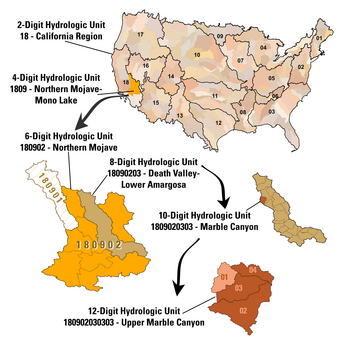
\includegraphics[width=\textwidth]{img/WBD_Base_HUStructure_small.png}
\end{column}
\end{columns}
\end{frame}

% ---------------------------------------------------------------- 15
\begin{frame}{MR violations are common; almost no MCL violations}
\pressum{violation_binary_days_panels_k2}
\takeaway{Nitrate MR 5.7\%, arsenic 3.7\%, IOC 4.3\% of utility-years. MCL violations: 12, 5, and 32 events across 1985--2005.}
\end{frame}

% ---------------------------------------------------------------- 16
\begin{frame}{Mining exposure in the sample}
\pressum{mining_exposure_covariates_k2}
\takeaway{On average 1.1 mines upstream and 1.1\% sulfur by weight; cumulative upstream production reaches 5.2 (10M ST) at the 99th percentile.}
\end{frame}

% ================================================================
\section{Does coal mining contaminate utility water?}
% ================================================================

\begin{frame}{Contaminant concentration summary statistics}
\pressum{6yr_huc02fe_inorg_val_sumstats_ravalli_2005_k2}
\end{frame}

% ---------------------------------------------------------------- 17
\begin{frame}{Design: cumulative production, measured concentrations}
\begin{equation*}
\textit{Concen}_{ct}= \beta\cdot\!\!\sum_{\tau=1985}^{t}\!\!\text{UpstreamCoalProd}_{c\tau} + \rho_c + HUC02_c\cdot\tau_t + \epsilon_{ct}
\end{equation*}
\begin{itemize}\small
    \item $\textit{Concen}_{ct}$: mean annual concentration at utility $c$, year $t$ (SYR2, 1998--2005).
    \item $\beta$: effect of 10 million additional cumulative short tons mined upstream since 1985.
    \item $\rho_c$: utility fixed effects. $HUC02_c\cdot\tau_t$: HUC02-specific year effects, absorbing watershed-wide industrial trends.
    \item SEs clustered at the utility level.
\end{itemize}
\medskip
\begin{itemize}
    \item Continuous treatment, \textbf{no control}: identification comes from relative exposure.
    \item Assumption: utilities with large upstream production changes would have trended like those with small ones. \backuplink{balancetest}{balance test on utility characteristics}
\end{itemize}
\end{frame}

% ---------------------------------------------------------------- 18
\begin{frame}{Mining raises contaminant levels}
\presreg{6yr_huc02fe_inorg_ravalli_2005_k2}
\takeaway{Nitrate $+$0.09 mg/L per 10M tons (***): 11.0\% of its mean. Selenium $+$0.0004 mg/L (**): 8.5\% of its mean. \textbf{Every reading in the sample stays under its MCL.} \backuplink{rob6yrannprod}{annual production}, \backuplink{rob6yrnmines}{number of mines}}
\end{frame}

% ================================================================
\section{Do utilities keep self-reporting?}
% ================================================================

\begin{frame}{The Acid Rain Program (``ARP") moved coal production for reasons unrelated to water quality}
\begin{columns}[T]
\begin{column}{0.44\textwidth}
\begin{itemize}\small

\item Adapt \textcite{stratford2015coalprod} ARP instrument for coal production to
address endogeneity of mining and utility characteristics.
\item 1990 Clean Air Act amendments cap SO$_2$ from power plants; Phase I deadline \textbf{1995}.
\item Power plants were 90\% of coal demand; switching to low sulfur coal was the main compliance response \parencite{lattanzio2022clean}.
\item High sulfur mines have limited ability to wash the sulfur out (bound to chemical structure).
\end{itemize}
\end{column}
\begin{column}{0.54\textwidth}
\includegraphics[width=\textwidth]{\outputdir/fig/coal_summary_plot.png}
\end{column}
\end{columns}
\end{frame}

\begin{frame}{Watershed coal sulfur content}
\presfig[0.78\textheight]{map_huc12_sulfur.png}
\end{frame}

\begin{frame}{Where coal production moved, 1985--2005}
\presfig[0.78\textheight]{proportionatecircleprod_diff_allminehuc12_1985_2005.png}
\end{frame}
% ---------------------------------------------------------------- 20
\begin{frame}{IV design: the ARP as a shifter of where coal is mined}
First stage:
\begin{equation*}
\begin{split}
\text{NumMines}_{ct} &= \alpha_0 + \alpha_1\text{NumFacility}_{ct} + \alpha_2\text{UpstreamCoalSulfur\%}_c \cdot \text{Post95}_t \\
&\quad + State_s \cdot Y_t + C_c + \nu_{ct}
\end{split}
\end{equation*}
Second stage:
\begin{equation*}
\text{Violation}_{vct} = \beta_0 + \beta_1\text{NumFacility}_{ct} + \gamma\widehat{\text{NumMines}}_{ct} + State_s \cdot Y_t + C_c + \epsilon_{ct}
\end{equation*}
\begin{itemize}\small
    \item $\text{Post95}_t = \mathbf{1}\{t \geq 1995\}$. Sulfur is time-invariant, so $C_c$ absorbs its level.
    \item Outcome: 1 if utility $c$ had a violation of type $v$ at any point in year $t$. Coefficients are in percentage points.
    \item SEs clustered at the utility level.
\end{itemize}
\end{frame}

% ---------------------------------------------------------------- 21
\begin{frame}{Shift in location of coal production w.r.t. sulfur}
\presfig[0.74\textheight]{scatterhuccoalsulfur_pooled.png}
\end{frame}

% ---------------------------------------------------------------- 22
\begin{frame}{First stage: high sulfur watersheds lost their mines}
\presreg[width=0.7\textwidth]{fs_dwnstrm_minevio_ivsum_k2}
%\takeaway{$F = 27.5$, above the 23.1 critical value of \cite{montielolea2013robust} for a 5\% test against 10\% worst-case bias, and well above the rule of thumb of 10 (\cite{staigerstock1997instrumental}).}
\takeaway{\backuplink{robfsannprod}{first stage for annual upstream coal production}}
\end{frame}

% ---------------------------------------------------------------- 23
\begin{frame}{Instrument validity}
\begin{itemize}\small
    \item \textbf{Independence.} The ARP is a national clean-air law set by national energy and emissions politics, not downstream utilities' water quality.
    \item \textbf{Exclusion.} Effect of instrumenting mining downstream of utility on utility behavior is not significant. \backuplink{updnfs}{upstream and downstream mines instrumented jointly}; \backuplink{kgridmrup}{MR violations}, \backuplink{kgridvisitup}{visits}, \backuplink{kgridenfup}{enforcement} across $k$.

    Utility characteristics are not predicted by instrument. \backuplink{exclfacilities}{full balance table}
    \item \textbf{Monotonicity.} A defier is a high-sulfur watershed that expanded \emph{because} its coal was high sulfur. Scrubber adoption costs more likely lead to lost market share rather than gain; low-cost high-sulfur regions that expand anyway are never-takers. 
    %Monotonicity is pairwise in sulfur, so low- and high-sulfur areas may respond in opposite directions (\cite{angrist1994identification}).
\end{itemize}
\end{frame}

% ---------------------------------------------------------------- 23a
\begin{frame}{Exclusion test: upstream and downstream mines instrumented jointly}
Two endogenous regressors, two instruments:
\begin{equation*}
\begin{split}
\text{Violation}_{vct} &= \gamma_U\,\widehat{\text{UpMines}}_{ct} + \gamma_D\,\widehat{\text{DownMines}}_{ct} \\
&\quad + \beta_1\text{NumFacility}_{ct} + State_s \cdot Y_t + C_c + \epsilon_{ct}
\end{split}
\end{equation*}
\begin{itemize}\small
    \item Instruments: $\text{Post95}_t \times \text{UpstreamSulfur\%}_c$ and $\text{Post95}_t \times \text{DownstreamSulfur\%}_c$.
    \item Downstream mines: coal mines within two watersheds \textbf{downstream} of the intake. Their runoff cannot reach the intake.
    \item If the ARP affects utilities only through upstream mining, $\gamma_D = 0$.
    \item A nonzero $\gamma_D$ would signal that the sulfur $\times$ post-1995 shift reaches utilities through another channel (local economy, regulator attention).
\end{itemize}
\end{frame}

% ---------------------------------------------------------------- 23b
\begin{frame}{Joint first stage: each instrument moves its own mines}
\hypertarget{updnfs}{}
\presreg[width=0.8\textwidth]{fs_dwnstrm_minevio_ivsum_k2updn}
\takeaway{Upstream sulfur predicts upstream mine loss ($F = 24.7$); downstream sulfur predicts downstream mine loss ($F = 18.3$). With utility and year fixed effects: $F = 20.0$ and $17.5$.}
\end{frame}

% ---------------------------------------------------------------- 23c
\begin{frame}{Downstream mines do not predict MR violations}
\hypertarget{updnmr}{}
\presreg{2sls_dwnstrm_minevio_mr_ivsum_binvio_k2updn}
\takeaway{The downstream 2SLS coefficient is insignificant in every column, and also in the combined, MCL, visit, and enforcement tables (29 of 29 columns). Confidence intervals are wide, and the upstream coefficient loses significance too. \backuplink{updnallcat}{combined}, \backuplink{updnmcl}{MCL}, \backuplink{updnvisit}{visits}, \backuplink{updnenf}{enforcement}, \backuplink{updnbal}{balance}, \backuplink{updnmrannprod}{annual production}}
\end{frame}

% ---------------------------------------------------------------- 23d
\begin{frame}{Event study: reduced form by year}
\begin{equation*}
\begin{split}
Y_{ct} &= \sum_{s \neq 1994} \delta_s \,\mathbf{1}\{t = s\} \times \text{UpstreamSulfur\%}_c \\
&\quad + \beta_1\text{NumFacility}_{ct} + State_s \cdot Y_t + C_c + \epsilon_{ct}
\end{split}
\end{equation*}
\begin{itemize}\small
    \item $\delta_s$: effect of 1 pp more upstream sulfur on outcome $Y$ in year $s$, relative to 1994, the year before ARP Phase I.
    \item Parallel trends: $\delta_{1985}=\dots=\delta_{1993}=0$, tested jointly.
    \item Post $-$ pre: mean of $\delta_s$ after 1995 minus mean before, the event-study analogue of the pooled reduced form.
\end{itemize}
\end{frame}

% ---------------------------------------------------------------- 23e
\begin{frame}{Event study: pre-1995 trends}
\hypertarget{eshead}{}
\presfig[0.72\textheight]{es_rf_headline_k2.png}
\takeaway{MCL violations and formal enforcement have flat pre-periods. MR violations rise in 1988--1991 and return to zero by 1994; after 1995 they sit near $+2$ pp. \backuplink{esmr}{MR by contaminant}, \backuplink{esall}{all outcomes}}
\end{frame}

% ---------------------------------------------------------------- 23f
\begin{frame}{Event study: joint pre-trend tests, violations}
\hypertarget{estable}{}
\presreg{es_rf_pretrend_vio_k2}
\end{frame}

% ---------------------------------------------------------------- 23g
\begin{frame}{Event study: joint pre-trend tests, visits and enforcement}
\presreg{es_rf_pretrend_visenf_k2}
\end{frame}

% ---------------------------------------------------------------- 24
\begin{frame}{Mining makes utilities stop reporting}
\presreg{2sls_dwnstrm_minevio_mr_ivsum_binvio_k2}
\takeaway{Base rates of nitrates, arsenic, and IOC are 5.7\%, 3.7\%, and 4.3\%. OLS estimates are far smaller --- consistent with negative omitted variable bias, as expected if poorly performing utilities (more MR violations) are protected from mine siting (fewer mines). \backuplink{robmrannprod}{annual upstream coal production}, \backuplink{eshead}{event study}}
\end{frame}

% ---------------------------------------------------------------- 26
\begin{frame}{Reporting cost, not concealment}
\begin{itemize}\small
    \item Nitrate rules require \textbf{more frequent monitoring} once a reading exceeds 50\% of the MCL --- a discrete jump in $c$, with no jump in the penalty for under-reporting and no MCL.
    \item Exceedance risk is held fixed (Channel B = 0), reporting cost increases (Channel A $\geq 0$).
\end{itemize}
\presreg{mr_concentration_lag_ols_k2}
\takeaway{Descriptive, not causal --- read the sign, not the magnitude. Utilities under-report when self-reporting gets expensive, not to conceal exceedances.}
\end{frame}

% ================================================================
\section{How do regulators respond?}
% ================================================================

% ---------------------------------------------------------------- 28
\begin{frame}{Enforcement does not counteract under-reporting}
\presreg{h3_inf_formal_d12_k2}
\takeaway{One more upstream mine reduces formal enforcement by 3.4 pp with utility and year fixed effects alone (significant), but the effect loses significance once state $\times$ year fixed effects are added. \backuplink{robenfannprod}{annual upstream coal production}}
\end{frame}

% ---------------------------------------------------------------- 29
\begin{frame}{The regulator increases inspections, not enforcement}
\presreg{h2_snsv_d12_k2}
\takeaway{Inspection visits rise significantly ($+$2.1 pp). Regulators do not systematically step up the visit types tied to sanctions. Visits would reveal concealment and be associated with higher penalties. \backuplink{robvisitannprod}{annual upstream coal production}}
\end{frame}

% ---------------------------------------------------------------- 30
\begin{frame}{Conclusion}
\begin{itemize}\small
    \item Exogenous contamination raises the cost of self-reporting, and self-reporting falls --- \textbf{even when utilities remain below MCL}.
    \item Under-reporting due to cost avoidance, rather than concealing a contamination violation.
    \item Regulators' inspection visits rise significantly --- substituting for utility self-reporting.
    \item Enforcement response is mixed and fixed-effects-sensitive: formal action falls with baseline fixed effects but loses significance once state $\times$ year effects are added.
    \item \textbf{Policy.} Tightening MCLs does nothing if nobody tests. Raising self-reporting penalties could reduce under-reporting.
    %\item \textbf{Policy.} Tightening MCLs does nothing if nobody tests. By Proposition 3 the binding lever is the price of \emph{not} reporting where source water is impaired, and it is not currently being pulled (\cite{malik1993self}; \cite{harford1987self}).
    \item Open question: whether regulator monitoring is more efficient than self-reporting.
\end{itemize}
\vfill
\centering \small ek559@cornell.edu
\end{frame}

% ================================================================
% Appendix
% ================================================================
\begin{frame}
\vfill
\centering
\begin{beamercolorbox}[sep=8pt,center,shadow=true,rounded=true]{title}
\usebeamerfont{title}Appendix\par
\end{beamercolorbox}
\vfill
\end{frame}

\begin{frame}{Appendix: combined MR and MCL violations}
\presreg{2sls_dwnstrm_minevio_allcat_ivsum_binvio_k2}
\takeaway{The combined effect mirrors the MR effect: nitrate 3.9--5.1 pp, arsenic 4.0--4.9 pp, IOC 3.1--4.6 pp across the two fixed-effects specifications. \backuplink{roballcatannprod}{annual upstream coal production}, \backuplink{robmclannprod}{MCL violations, annual production}}
\end{frame}

\begin{frame}{Appendix: instrument balance on intake facilities}
\hypertarget{exclfacilities}{}
\presreg{exclusion_test_num_facilities_k2}
\end{frame}

\begin{frame}{Appendix: balance test on utility characteristics}
\hypertarget{balancetest}{}
\presreg[max width=\textwidth, max totalheight=0.68\textheight]{pt_balance_6yr_k2}
\takeaway{Observable characteristics jointly predict continuous upstream production only without state fixed effects (p=0.029) and lose significance once state fixed effects are added (p=0.461), as in the main specification. The joint test on the binary presence of upstream mining stays significant with or without state fixed effects.}
\end{frame}

\begin{frame}{Appendix: exclusion placebo, MR violations across $k$}
\hypertarget{kgridmrup}{}
\presfig[0.66\textheight]{kgrid_mr_upstream_of_mine_coefs.png}
\takeaway{For utilities upstream of a mine --- where mining cannot reach the intake hydrologically --- OLS estimates on MR violations are positive and significant at every $k$. In the reduced form and 2SLS, nitrate estimates are significant for $k \geq 3$, while arsenic and inorganic chemical estimates are significant only at $k=1$.}
\end{frame}

\begin{frame}{Appendix: exclusion placebo, visits across $k$}
\hypertarget{kgridvisitup}{}
\presfig[0.68\textheight]{kgrid_visit_upstream_of_mine_coefs.png}
\takeaway{For utilities upstream of a mine, inspection visits rise significantly at nearly every $k$, sanitary visits at $k=1$ and $k \geq 4$, and sample collection visits at several radii; technical assistance and enforcement visits are mostly insignificant.}
\end{frame}

\begin{frame}{Appendix: exclusion placebo, enforcement across $k$}
\hypertarget{kgridenfup}{}
\presfig[0.76\textheight]{kgrid_enf_upstream_of_mine_coefs.png}
\takeaway{Enforcement actions show no consistent pattern for utilities upstream of a mine at any choice of $k$, supporting the exclusion restriction.}
\end{frame}

% ---------------------------------------------------------------- robustness: regressor swap
\begin{frame}{Robustness: concentrations and annual upstream production}
\hypertarget{rob6yrannprod}{}
\presreg{6yr_huc02fe_inorg_ravalli_2005_k2annprod}
\takeaway{Annual production (1M short tons) replaces cumulative production. Arsenic ($+$0.0032 mg/L, ***) and nitrate ($+$0.079 mg/L, *) rise within one watershed upstream; nitrate also rises within two ($+$0.061 mg/L, ***). Barium and selenium are not significant.}
\end{frame}

\begin{frame}{Robustness: concentrations and the number of upstream mines}
\hypertarget{rob6yrnmines}{}
\presreg{6yr_huc02fe_inorg_ravalli_2005_k2nmines}
\takeaway{With the contemporaneous count of upstream mines as the regressor, only barium within one watershed upstream is marginally significant.}
\end{frame}

\begin{frame}{Robustness: first stage for annual upstream coal production}
\hypertarget{robfsannprod}{}
\presreg[width=0.6\textwidth]{fs_dwnstrm_minevio_ivsum_k2annprod}
\takeaway{High-sulfur watersheds lost 0.10M short tons per percentage point of sulfur after 1995. $F = 11.8$ with state $\times$ year fixed effects, $18.1$ with utility and year fixed effects.}
\end{frame}

\begin{frame}{Robustness: MR violations and annual upstream production}
\hypertarget{robmrannprod}{}
\presreg{2sls_dwnstrm_minevio_mr_ivsum_binvio_k2annprod}
\takeaway{One million more short tons mined upstream raises MR violations by 15--21 pp, significant in all six columns.}
\end{frame}

\begin{frame}{Robustness: combined violations and annual upstream production}
\hypertarget{roballcatannprod}{}
\presreg{2sls_dwnstrm_minevio_allcat_ivsum_binvio_k2annprod}
\end{frame}

\begin{frame}{Robustness: MCL violations and annual upstream production}
\hypertarget{robmclannprod}{}
\presreg{2sls_dwnstrm_minevio_mcl_ivsum_binvio_k2annprod}
\takeaway{As with mine counts, MCL violations do not respond to upstream production.}
\end{frame}

\begin{frame}{Robustness: enforcement and annual upstream production}
\hypertarget{robenfannprod}{}
\presreg{h3_inf_formal_d12_k2annprod}
\takeaway{Formal enforcement falls by 13.8 pp per million short tons with utility and year fixed effects (***); informal enforcement and no enforcement are not significant.}
\end{frame}

\begin{frame}{Robustness: visits and annual upstream production}
\hypertarget{robvisitannprod}{}
\presreg{h2_snsv_d12_k2annprod}
\takeaway{Inspection visits rise by 10.5 pp per million short tons (*); other visit types are not significant.}
\end{frame}

% ---------------------------------------------------------------- two-instrument appendix
\begin{frame}{Appendix: joint instruments, combined violations}
\hypertarget{updnallcat}{}
\presreg{2sls_dwnstrm_minevio_allcat_ivsum_binvio_k2updn}
\end{frame}

\begin{frame}{Appendix: joint instruments, MCL violations}
\hypertarget{updnmcl}{}
\presreg{2sls_dwnstrm_minevio_mcl_ivsum_binvio_k2updn}
\end{frame}

\begin{frame}{Appendix: joint instruments, visits}
\hypertarget{updnvisit}{}
\presreg{h2_snsv_d12_k2updn}
\takeaway{\backuplink{updnvisitannprod}{annual production}}
\end{frame}

\begin{frame}{Appendix: joint instruments, enforcement}
\hypertarget{updnenf}{}
\presreg{h3_inf_formal_d12_k2updn}
\takeaway{\backuplink{updnenfannprod}{annual production}}
\end{frame}

\begin{frame}{Appendix: joint instruments, balance on intake facilities}
\hypertarget{updnbal}{}
\presreg{exclusion_test_num_facilities_k2updn}
\end{frame}

\begin{frame}{Robustness: joint instruments, MR violations and annual production}
\hypertarget{updnmrannprod}{}
\presreg{2sls_dwnstrm_minevio_mr_ivsum_binvio_k2updnannprod}
\takeaway{Downstream production is insignificant in all six columns, but the test has low power: the joint first-stage $F$ is 5.5 for downstream production, and 11.3 (utility and year fixed effects) or 5.9 (state $\times$ year fixed effects) for upstream production.}
\end{frame}

\begin{frame}{Robustness: joint instruments, enforcement and annual production}
\hypertarget{updnenfannprod}{}
\presreg{h3_inf_formal_d12_k2updnannprod}
\takeaway{Downstream production is insignificant in all six columns. Joint first-stage $F$ is 5.5 downstream, and 5.9--11.3 upstream.}
\end{frame}

\begin{frame}{Robustness: joint instruments, visits and annual production}
\hypertarget{updnvisitannprod}{}
\presreg{h2_snsv_d12_k2updnannprod}
\takeaway{Downstream production is insignificant for every visit type. Joint first-stage $F$ is 5.5 downstream and 5.9 upstream.}
\end{frame}

% ---------------------------------------------------------------- event-study appendix
\begin{frame}{Appendix: event study, MR violations by contaminant}
\hypertarget{esmr}{}
\presfig[0.55\textheight]{es_rf_mr_binvio_k2.png}
\takeaway{Nitrate, arsenic, and IOC MR violations all rise in 1988--1991 relative to 1994 (pre-1995 joint $p \le 0.01$) and are flat after 1995.}
\end{frame}

\begin{frame}{Appendix: event study, any violation}
\hypertarget{esall}{}
\presfig[0.55\textheight]{es_rf_allcat_binvio_k2.png}
\end{frame}

\begin{frame}{Appendix: event study, MCL violations}
\presfig[0.55\textheight]{es_rf_mcl_binvio_k2.png}
\end{frame}

\begin{frame}{Appendix: event study, regulator visits}
\presfig[0.72\textheight]{es_rf_h2_snsv_k2.png}
\end{frame}

\begin{frame}{Appendix: event study, enforcement}
\presfig[0.72\textheight]{es_rf_h3_enf_k2.png}
\end{frame}

\begin{frame}{Appendix: who appears in the Six-Year Review}
\pressum{syr2_mr_comparison_k2}
\takeaway{Utilities with SYR2 readings are 7--14 pp more likely to ever incur an MR violation. The concentration sample over-represents the more negligent utilities, so it is not selected toward clean systems.}
\end{frame}

\begin{frame}{Appendix: enforcement and visits in the panel}
\pressum{enforcement_visit_type_panels_k2}
\takeaway{Enforcement responds to violations --- any enforcement rises from 21\% overall to 71\% in MR years --- but sanitary visits are no more likely in MR years than in any other year.}
\end{frame}

\begin{frame}{Appendix: residualized first stage}
\presfig[0.72\textheight]{first_stage_scatter_dwnstrm.png}
\end{frame}

\begin{frame}{Appendix: sample watersheds}
\presfig[0.72\textheight]{map_huc12_main_sample.png}
\end{frame}

\begin{frame}{Appendix: Corollary 1, statement and proof}
\scriptsize
Write the share of types under-reporting as $h(\theta,m) = 1 - G(c^*(\theta);m)$, with cutoff $c^*(\theta) = t - (r-ps)\,q(a_{SR}(\theta))$, so that
\[
\frac{\partial MR}{\partial m} = \underbrace{\int_0^{\bar\theta}\!\frac{\partial h(\theta,m)}{\partial m}\,f(\theta;m)\,d\theta}_{\text{A: cost}} \;+\; \underbrace{\int_0^{\bar\theta}\! h(\theta,m)\,\frac{\partial f(\theta;m)}{\partial m}\,d\theta}_{\text{B: composition}}.
\]
\textbf{Corollary 1.} If $q(a_{SR}(\theta)) \equiv \bar q$ on $(0,\bar\theta)$, then $\partial MR/\partial m = -\,\partial G(\bar c;m)/\partial m \ge 0$, where $\bar c = t-(r-ps)\bar q$.
\smallskip

\textit{Proof.} The cutoff is then type-invariant, $c^*(\theta) \equiv \bar c$, so $h(\theta,m) = 1-G(\bar c;m)$ does not vary with $\theta$ and comes outside both integrals. The limits $0$ and $\bar\theta$ do not depend on $m$, so by Leibniz's rule
\[
\text{B} = \big[1-G(\bar c;m)\big]\,\frac{d}{dm}\!\left[\int_0^{\bar\theta}\! f(\theta;m)\,d\theta\right] = \big[1-G(\bar c;m)\big]\,\frac{d}{dm}[1] = 0,
\]
since $f(\cdot\,;m)$ is a density for every $m$. Channel A collapses to $-\,\partial G(\bar c;m)/\partial m \ge 0$, because contamination shifts reporting costs up. $\square$
\smallskip

\textbf{Why it matters.} Channel B is the concealment margin: it operates only if contamination reallocates mass toward types whose exceedance risk, and hence whose cutoff, differs. Shut it down and any remaining rise in under-reporting is avoidance of the reporting technology itself. The 50\%-of-MCL nitrate step is the empirical counterpart --- monitoring frequency jumps, the sanction schedule does not, and readings are nowhere near the limit.
\end{frame}

% ================================================================
% Mine accident instruments (run_k2_accident_iv_tables.r)
% ================================================================
\section{Robustness: mine accident instruments}

\begin{frame}{Mine accident instruments: estimating equations}
\hypertarget{accideq}{}
Second stage:
\begin{equation*}
\begin{split}
\text{Violation}_{vct} &= \gamma_U\,\widehat{\text{UpProd}}_{ct} + \gamma_D\,\widehat{\text{DownProd}}_{ct} \\
&\quad + \beta_1\text{NumFacility}_{ct} + State_s \cdot Y_t + C_c + \epsilon_{ct}
\end{split}
\end{equation*}
First stage, for each $P \in \{\text{UpProd}, \text{DownProd}\}$:
\begin{equation*}
\begin{split}
P_{ct} &= \pi_1^P\,\text{UpAcc}_{ct} + \pi_2^P\,\text{UpSulfur\%}_c \cdot \text{Post95}_t \\
&\quad + \pi_3^P\,\text{DownAcc}_{ct} + \pi_4^P\,\text{DownSulfur\%}_c \cdot \text{Post95}_t \\
&\quad + \alpha_1\text{NumFacility}_{ct} + State_s \cdot Y_t + C_c + \nu_{ct}
\end{split}
\end{equation*}
\begin{itemize}\small
    \item Prod: annual coal production (1M short tons) within two watersheds upstream / downstream of the intake. Acc: MSHA accident, injury, and illness reports at those mines (units of 10).
    \item Columns add instruments in order: (1) UpAcc; (2) $+$ UpSulfur $\times$ Post95; (3) $+$ DownAcc, with DownProd as a second endogenous regressor; (4) $+$ DownSulfur $\times$ Post95.
    \item Outcomes are 0/1; coefficients in percentage points. SEs clustered at the utility level.
\end{itemize}
\end{frame}

\begin{frame}{Mine accident instruments: MR violations}
\presreg{2sls_dwnstrm_minevio_mr_ivsum_binvio_k2accprog}
\takeaway{Upstream accidents strongly predict upstream production ($F = 77.0$ in column 1). With accidents in the instrument set, the upstream 2SLS estimate on MR violations is near zero and insignificant (IOC $-1.11$ to $-0.47$), well below the sulfur-only estimate of 15.02. Downstream production is insignificant; its first-stage $F$ falls to 8.5 in column 4.}
\end{frame}

\begin{frame}{Mine accident instruments: enforcement}
\presreg{h3_inf_formal_d12_k2accprog}
\takeaway{Upstream production raises formal enforcement only in column 1 (1.71 pp, *). No other upstream or downstream coefficient is significant.}
\end{frame}

\begin{frame}{Mine accident instruments: regulator visits}
\presreg{h2_snsv_d12_k2accprog}
\takeaway{Upstream production has no significant effect on any visit type. Downstream production raises inspection visits (5.01 and 4.56 pp, **) and enforcement visits in column 4 (1.66 pp, *).}
\end{frame}

\begin{frame}[allowframebreaks]{References}
\printbibliography
\end{frame}

\end{document}
